\documentclass[10pt]{article}
\usepackage{../setup}
\usepackage{subfig}
\vspace{-8ex}
\date{}

\graphicspath{ {./figs/} }

\begin{document}

\title{\textbf{\Large{\textsc{ECE410:} Linear Control Systems}} \\ \Large{Lab 1 Report: Numerical Simulations of Dynamical Systems} \\ \textbf{\small{PRA102}}\vspace{-0.3cm}}
\author{Pranshu Malik, Varun Sampat \\ \footnotesize{1004138916}, \footnotesize{1003859602}\vspace{-3cm}}

\maketitle

\section{Introduction}
In this lab, we consider a pendulum-cart system with the control input, $u$, being the force imparted at the point of pivot, being the cart base, which is free to move along a frictionless rod. We consider the state of the system to be $\vec{x} = \rcvec{x_1 & x_2}^\intercal = \rcvec{\theta & \dot{\theta}}^\intercal$, where $\theta$ is the angle subtended by the pendulum rod against the vertically downwards axis. The pendulum has a mass, $M$, and is subject to gravity, $g$. The system, as a whole, has the following nonlinear dynamics:

\begin{figure}[!h]
\centering
\pendcartsimple
\caption{Pendulum-Cart system}
\end{figure}

\begin{equation*}
    \dot{\vec{x}} = f(\vec{x}, u) = \rcvec{ x_2 \\ \frac{-g \sin(x_1)}{l} \frac{-\cos(x_1)}{Ml}}
\end{equation*}

\section{Numerical Integration}
The system state evolution was determined numerically using \texttt{ode45} function in MATLAB. There were two initial conditions of interest:
\begin{equation*}
    \vec{x}_{0,1} = \rcvec{ 0\\ \sqrt{g/l} }\quad \text{and} \quad \vec{x}_{0,2} =  \rcvec{0\\1.99 \sqrt{g/l}}
\end{equation*}

Note, $x_1 = \theta$, and $x_2 = \dot{\theta}$. 
$\theta = 0$, but $\dot{\theta}$ is a non-zero value. In words, this is providing the pendulum with an initial velocity from its rest position (equilibrium at $\theta = 0$) at time $t = 0$.

\subsection{Graphs for initial condition $\vec{x}_{0,1}$}
\begin{figure}[ht]
    \centering
    \begin{minipage}[b]{0.45\textwidth}
        \centering
        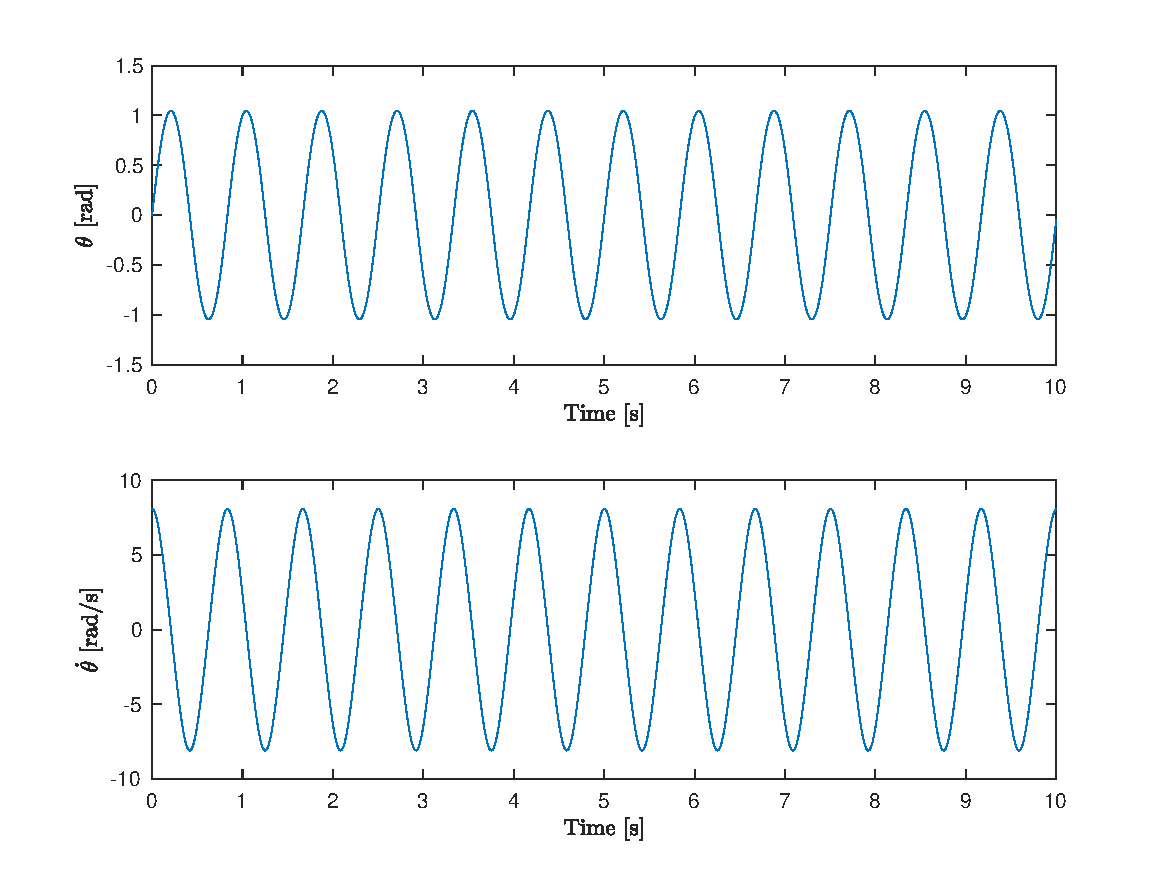
\includegraphics[width=1\linewidth]{lab1/figs/section3_x0_1_state_evolution.pdf}
        \captionof{figure}{state evolution for initial condition $\vec{x}_{0,1}$}    
    \end{minipage}
    \begin{minipage}[b]{0.45\textwidth}
        \centering
        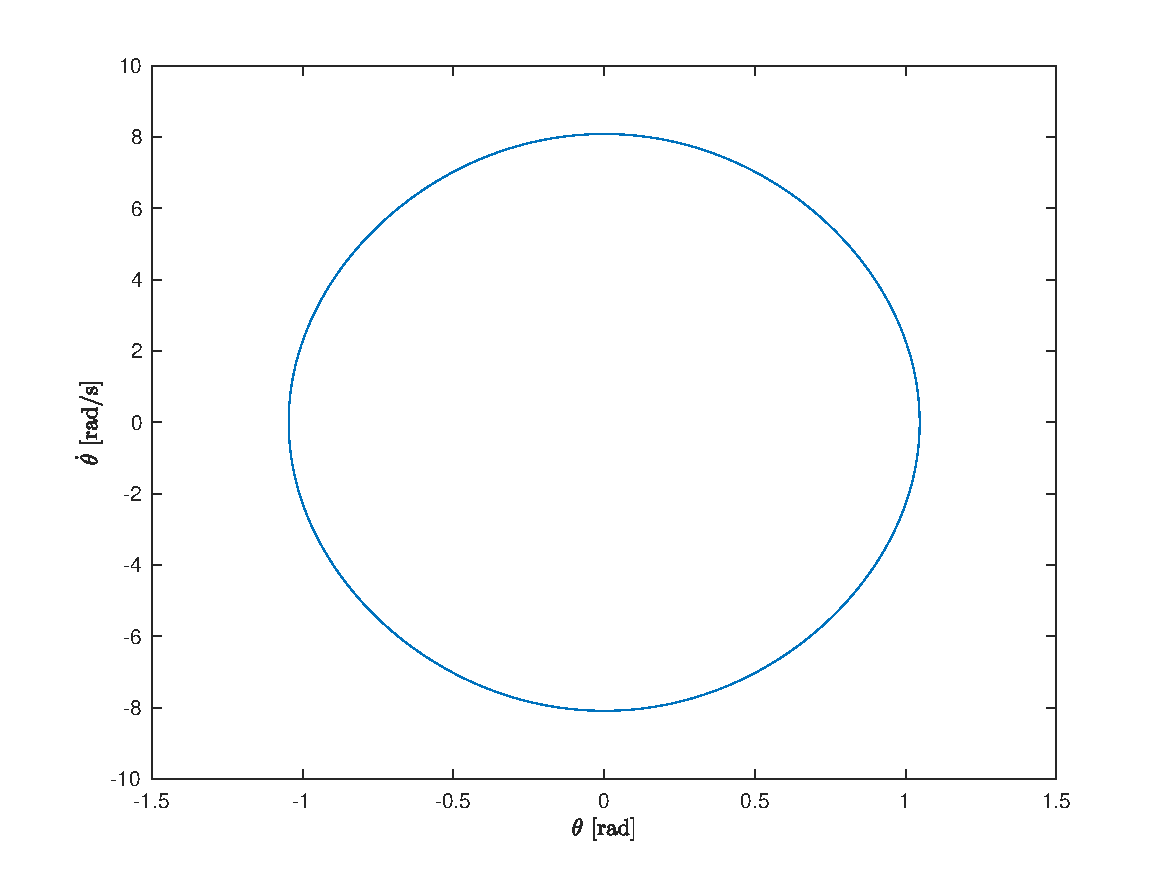
\includegraphics[width=1\linewidth]{lab1/figs/section3_x0_1_state_orbit.pdf}
        \captionof{figure}{State orbit for initial condition $\vec{x}_{0,1}$}
    \end{minipage}
    
    \label{figure:x_0_1_state_evolution}
\end{figure}
    
\subsection{Graphs for initial condition $\vec{x}_{0,2}$}
\begin{figure}[ht]
    \centering
    \begin{minipage}[b]{0.45\textwidth}
        \centering
        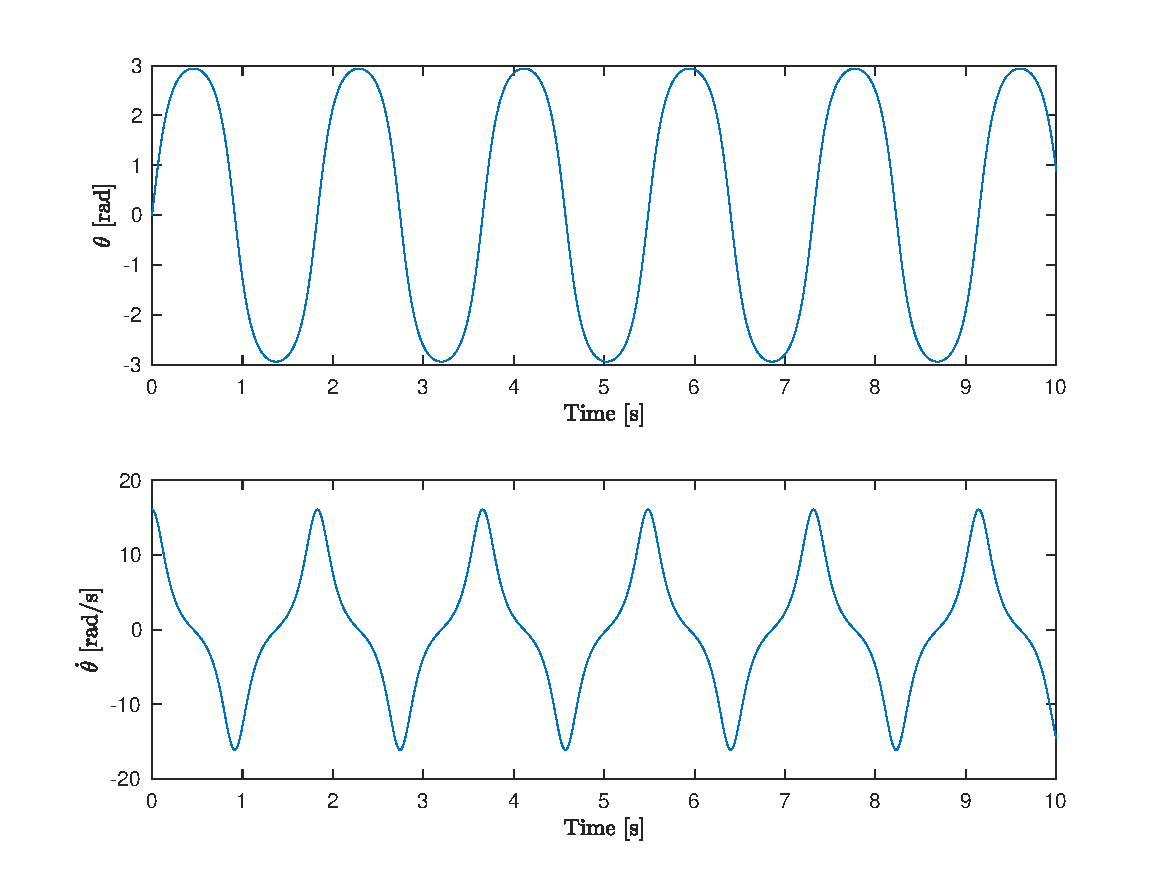
\includegraphics[width=1\linewidth]{lab1/figs/section3_x0_2_state_evolution.pdf}
        \captionof{figure}{state evolution for initial condition $\vec{x}_{0,2}$}    
    \end{minipage}
    \begin{minipage}[b]{0.45\textwidth}
        \centering
        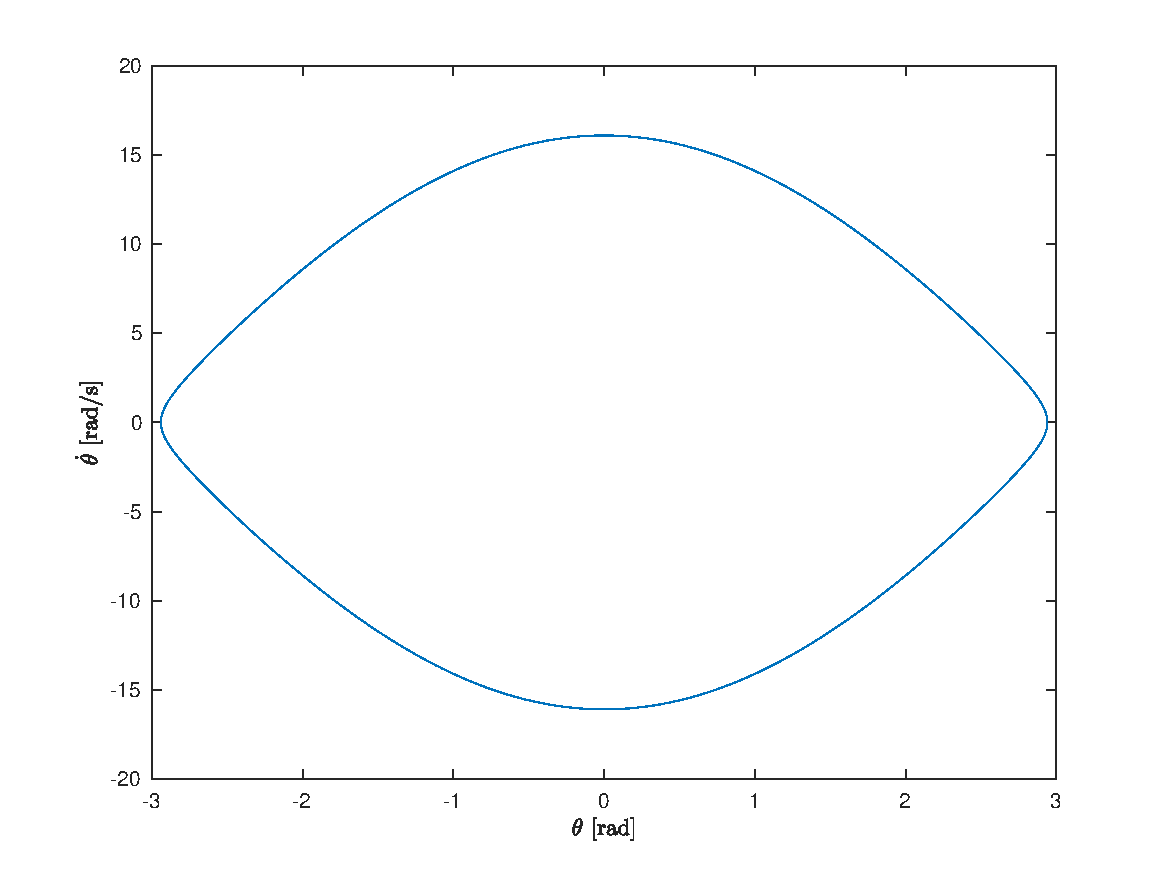
\includegraphics[width=1\linewidth]{lab1/figs/section3_x0_2_state_orbit.pdf}
        \captionof{figure}{State orbit for initial condition $\vec{x}_{0,2}$}
    \end{minipage}
    
    \label{figure:x_0_2_state_evolution}
\end{figure}

\subsection{Comparison/Analysis}
    The system response is clearly sinusoidal for the first initial condition and not the second. The frequency of the first initial condition is higher than the frequency of the second initial condition, on visual introspection. The state orbit for the first initial condition is a circle but for the second, it is more like an eye. 
    
    To understand the difference in the responses, it is important to identify what differentiates the initial conditions. The first condition basically injects a lower angular velocity (and hence, a lower linear velocity) than the second initial condition. Since no energy is lost here, the pendulum should sweep a higher angle for a higher initial velocity. This is seen in figures 3 and 5, where the \begin{math}
     max(\theta)_1 << max(\theta)_2
    \end{math}. Because initial condition 2 reaches a higher value of $\theta$ ($\approx$ 3 rad), one would expect a higher time period, which justifies a lower frequency than initial condition 1, that only goes up to $\approx$ 1 rad. 
    
    3 rad is $\approx$ $\pi$ which is 180 deg, which means physically speaking, the pendulum almost reaches the top. Looking at the state orbit graph for initial condition 2, it is almost making a complete revolution; $\theta$ covered is $\approx$ -3 rad to 3 rad. A higher initial velocity would lead to the pendulum making revolutions where the same value of $\theta$ would never repeat (ever increasing $\theta$!). 
    
    Recognize that the state evolution and state orbit responses/graphs are not unique to the initial conditions for this system. For example, the first initial condition could start with $\theta$ $\approx$ 1 rad and 0 initial velocity and the same system response would be obtained. 
    

\section{Symbolic Linearization}

\subsection{Equilibrium 1 $\vec{x}_1^*$}
    \begin{equation*}
         \vec{x}^* = \rcvec{0\\0}
         \quad
         \text{and}
         \quad
         \vec{u}^* = 0
    \end{equation*}

The resulting A, B matrices for this equilibrium point are:
\begin{equation*}
        A = 
        \begin{bmatrix}
        0 &1 \\ \frac{-g}{l} & 0
        \end{bmatrix}
        \quad
        \text{and}
        \quad
        B = 
        \begin{bmatrix}
        0\\ \frac{-1}{Ml}
        \end{bmatrix}
\end{equation*}

The C, D values for this equilibrium point are:
\begin{equation*}
    C = 
        \begin{bmatrix}
        1 & 0
        \end{bmatrix}
        \quad
        \text{and}
        \quad
        D = 
        \begin{bmatrix}
        0
        \end{bmatrix}
\end{equation*}

This matches the equations provided in the lab handout.
\subsection{Equilibrium 2 $\vec{x}_2^*$}
\begin{equation*}
        \vec{x}^* =
     \rcvec{\theta^* \\ 0}
     \quad
     \text{and}
     \quad
     \vec{u}^* = -Mg\tan(\theta^*) 
\end{equation*}

The resulting A, B matrices for this equilibrium point are:
\begin{equation*}
        A = 
        \begin{bmatrix}
        0 &1 \\ \frac{-g\cos(\theta^*)}{l} - g \frac{\sin(\theta^*) \tan(\theta^*)}{l} & 0
        \end{bmatrix}
\end{equation*}
Using $\tan(\theta) = \frac{\sin(\theta)}{\cos(\theta)}$, $A$ can be simplified as:
\begin{equation*}
        A =
        \begin{bmatrix}
        0 &1 \\ \frac{-g}{l\cos(\theta^*)} & 0
        \end{bmatrix}
        \quad
        \text{and}
        \quad
        B = 
        \begin{bmatrix}
            0\\ \frac{-\cos(\theta^*)}{Ml}
        \end{bmatrix}
\end{equation*}

$A$ matches that of the textbook. $B$ however, contains the m (mass) term whereas the textbook has no mention of mass. If m = 1 is plugged into the equations derived above, the same equations as the textbook will be obtained. Also note, setting $\theta = 0$ here results in the same matrices derived in 3.1 ($\tan(0)$ is 0, resulting in no effect caused by the input force $u$).

\section{Symbolic Expression to Numerical Integration}
Linearization was done about $\vec{x}_1^*$ defined in section 3.1.

\subsection{Graphs for initial condition $\vec{x}_{0,1}$}

\begin{figure}[ht]
    \centering
    \begin{minipage}[b]{0.45\textwidth}
        \centering
        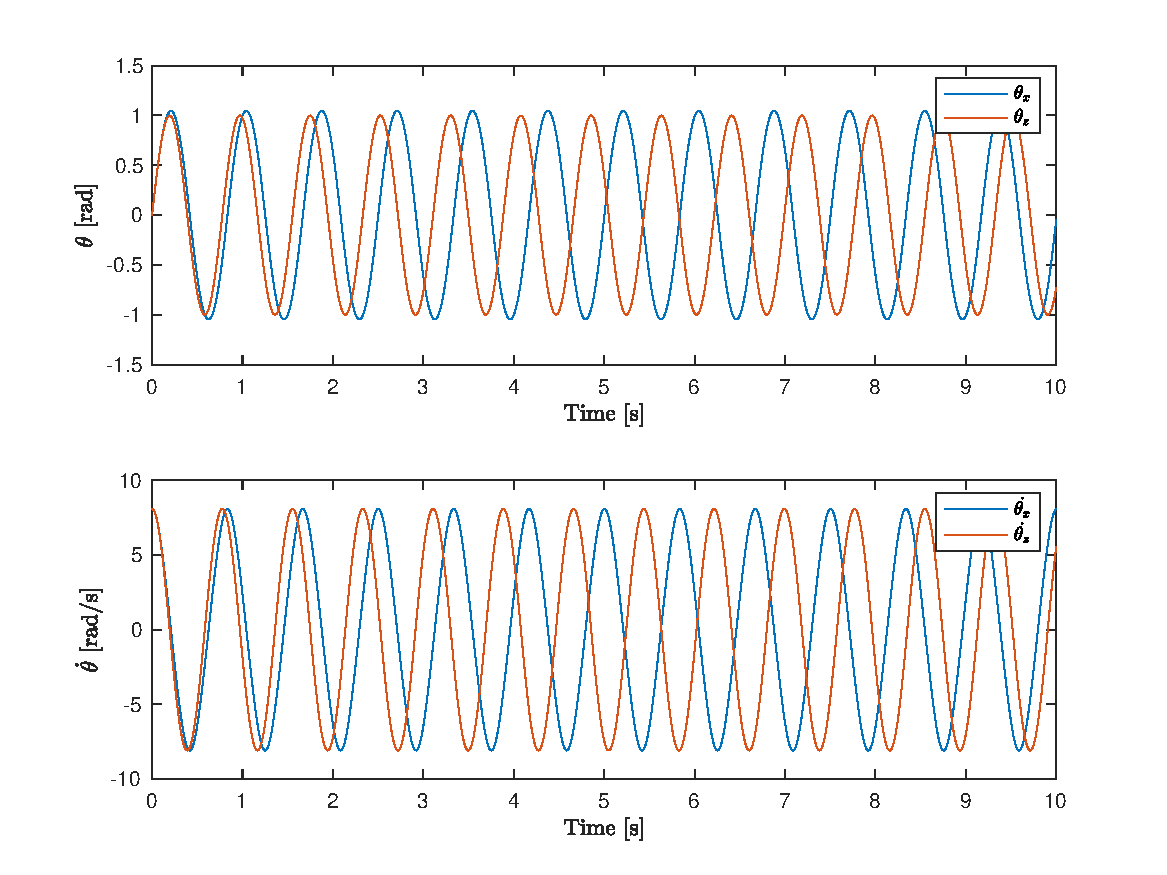
\includegraphics[width=1\linewidth]{lab1/figs/section5_X0_1_state_evolution.pdf}
        \captionof{figure}{state evolution for initial condition $\vec{x}_{0,1}$}    
    \end{minipage}
    \begin{minipage}[b]{0.45\textwidth}
        \centering
        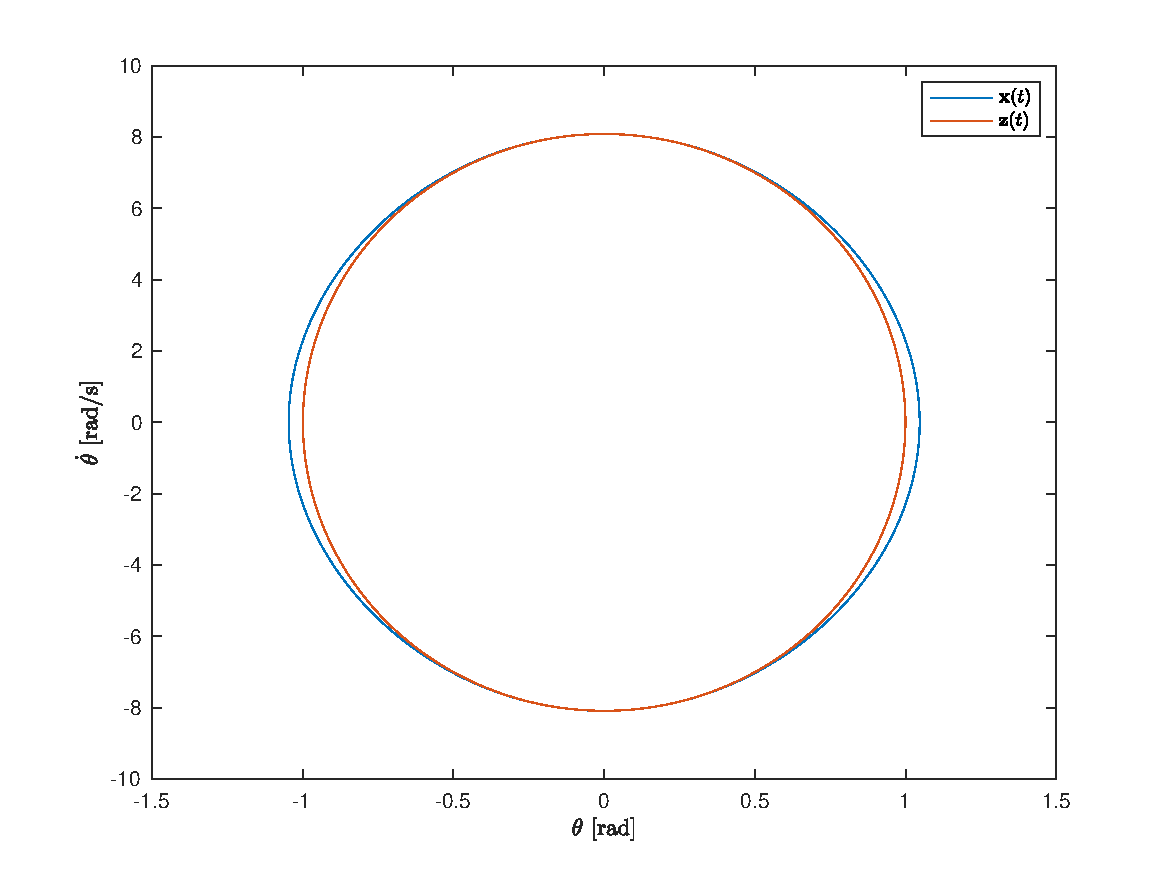
\includegraphics[width=1\linewidth]{lab1/figs/section5_X0_1_state_orbit.pdf}
        \captionof{figure}{State orbit for initial condition $\vec{x}_{0,1}$}
        \label{fig:test2}
    \end{minipage}
    
    \label{figure:x_0_1_state_evolution}
\end{figure}
    In figure 7, it can be seen that the state space coverage is somewhat similar for the linear and non-linear models. The range for $\dot{\theta}$ is the same for both the models, but the range for $\theta$ is slightly different. The non-linear model covers an additional range, which is when the linear model is not effective anymore.
    
    This additional coverage for $\theta$ is what introduces a phase shift-like  effect seen in time response of the system. Both the non-linear and linear model simulations have the same initial condition, so as long as they cover the same angle, the linear model is able to follow the actual system. However, once outside of the operating region, the linear model reaches a maximum and starts heading back to the equilibrium position. In this time, the non-linear part covers an addition $\theta$ and hence starts deviating from the linear system. 
    
    Basically, since the range for $\theta$ in the non-linear system is higher (but ever so slightly!), the frequency is ever so slightly lower than the linear model, leading to the discrepancies. A mathematical perspective that can help understand this drawback is the relationship between $f(x) = \sin(x)$ and $f(x) = x$. The linear model assumes $\sin(x) \approx x$, but this assumption is only valid at a certain range near $x \approx 0$, which explains the deviation observed in the figures above. 
    
\subsection{Graphs for initial condition $\vec{x}_{0,2}$}
\begin{figure}[ht]
    \centering
    \begin{minipage}[b]{0.45\textwidth}
        \centering
        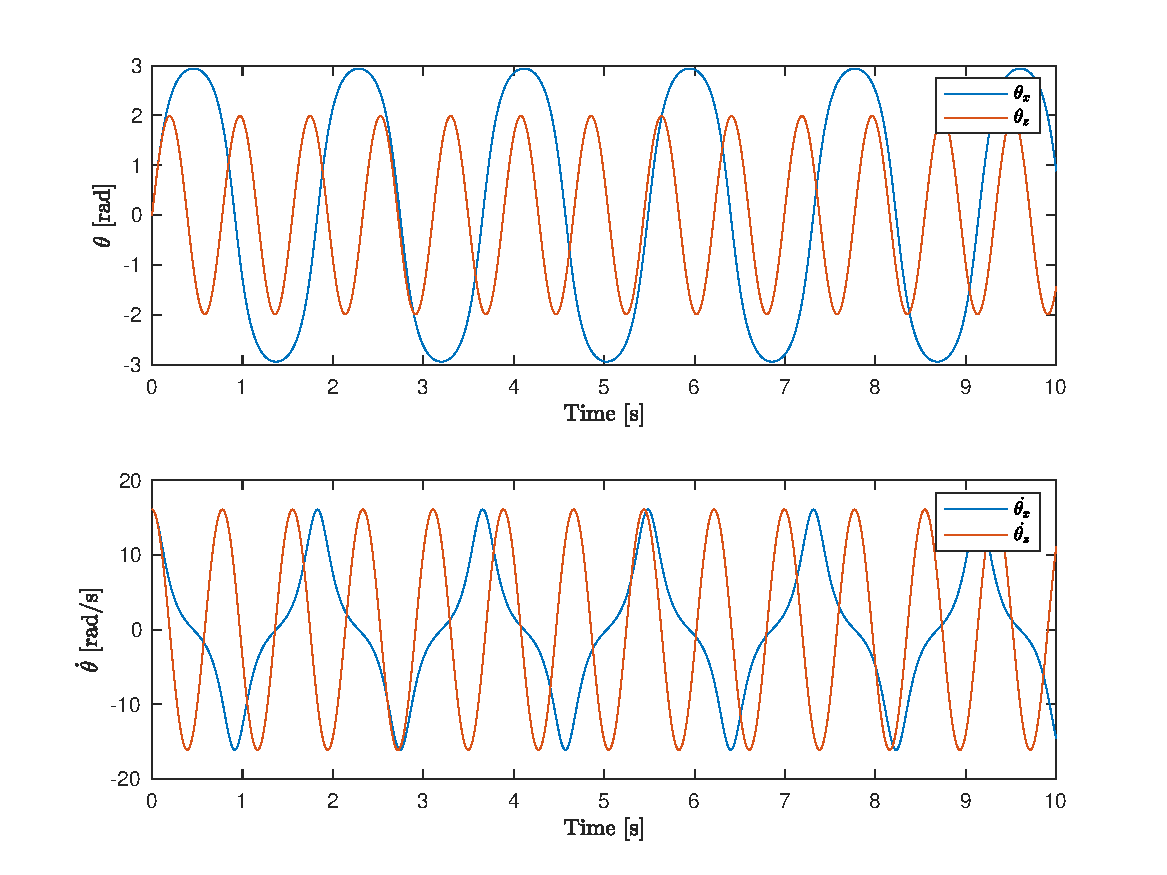
\includegraphics[width=1\linewidth]{lab1/figs/section5_X0_2_state_evolution.pdf}
        \captionof{figure}{State Evolution for initial condition $\vec{x}_{0,2}$}    
    \end{minipage}
    \begin{minipage}[b]{0.45\textwidth}
        \centering
        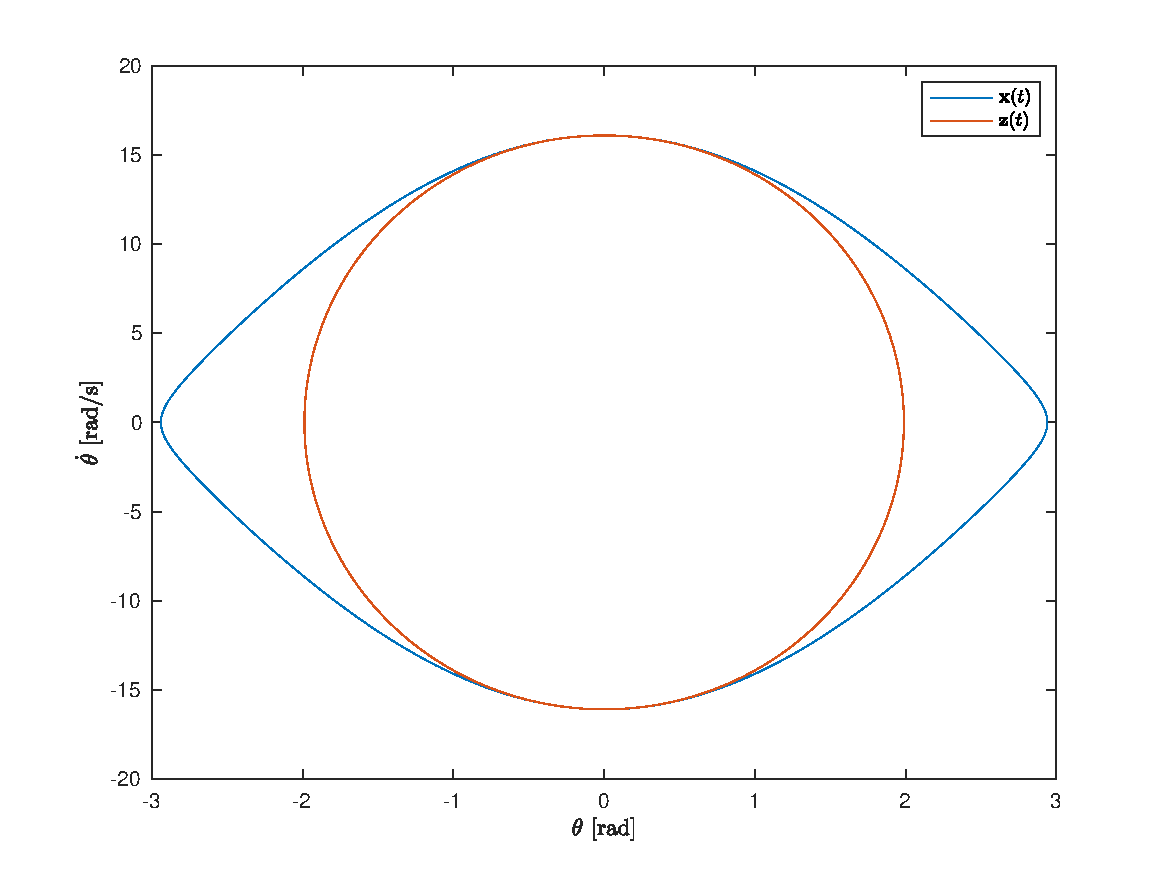
\includegraphics[width=1\linewidth]{lab1/figs/section5_X0_2_state_orbit.pdf}
        \captionof{figure}{State orbit for initial condition $\vec{x}_{0,2}$}
    \end{minipage}
    
    \label{figure:x_0_2_state_evolution}
\end{figure}

Here, the deviation talked about before is introduced earlier in the system. Recall that the law of conservation of energy must hold in the non-linear system, implying that every point on the state orbit has the same energy (KE + PE = constant). The linear model however, does not obey the law of conservation of energy, which explains the difference in the state orbits as well as the differences in the frequencies and amplitude. While this conflict existed in the first initial condition as well, in this condition, the differences are amplified and expose the pitfall of the linear model. However, looking at the scales of the axes for the state orbits, it can be seen that the tracking error is actually small. 

\subsection{Summary}
Initial condition $\vec{x}_{0,2}$ injects a higher kinetic energy than initial condition $\vec{x}_{0,1}$. This disparity led to the linear model working more accurately for $\vec{x}_{0,1}$ and observed a clear incapability to follow the system for $\vec{x}_{0,2}$. In summary, the further the pendulum goes away from the equilibrium point, the worse the linear model gets at predicting the true motion of the system.

\section{LTI Representations}
% plot eigenvalues and poles of the system!!!! Do it using pgf plots, matlab not nice for that.
Eigenvalues of A:
\begin{equation*}
    \sigma(A) = \{8.0870i, -8.0870i\}
\end{equation*}

Eigenvectors obtained for the corresponding eigenvalues
\begin{equation*}
    V = [\vec{v}|\vec{v}^*] = \begin{bmatrix}
    -0.1227i & 0.1227i\\ 0.9924 & 0.9924 
    \end{bmatrix}
\end{equation*}

The transfer function obtained for the linearized pendulum system
\begin{equation*}
G(s) = \frac{-33.33}{s^2+65.4} = \frac{-33.33}{(s-8.0870i)(s+8.0870i)} 
\end{equation*}

\subsection{Analysis}
The poles of the transfer function are equal to the eigenvalues of A. This implies that there are no pole-zero cancellations taking place. Additionally, the poles are purely imaginary, implying that the system response is purely sinusoidal (no decay). Looking at the system from a mathematical perspective, this makes sense since the differential equations that govern the system do not have any damping factor. Physically, there are no energy losses in the system, so the energy that is injected in the system infinitely oscillates between kinetic energy and potential energy. 

\subsubsection{Internal Stability}
Because the poles are purely imaginary, the system cannot be asymptotically stable. Consider $\theta_0 = \pi/4$, then the pendulum would infinitely oscillate. However, for any starting internal state ($x_0$), the linear system will always produce a bounded sinusoidal output, implying that the system is stable. This is mathematically backed by equal algebraic and geometric multiplicities of the eigenvalues.

\begin{figure}[ht]
    \centering
        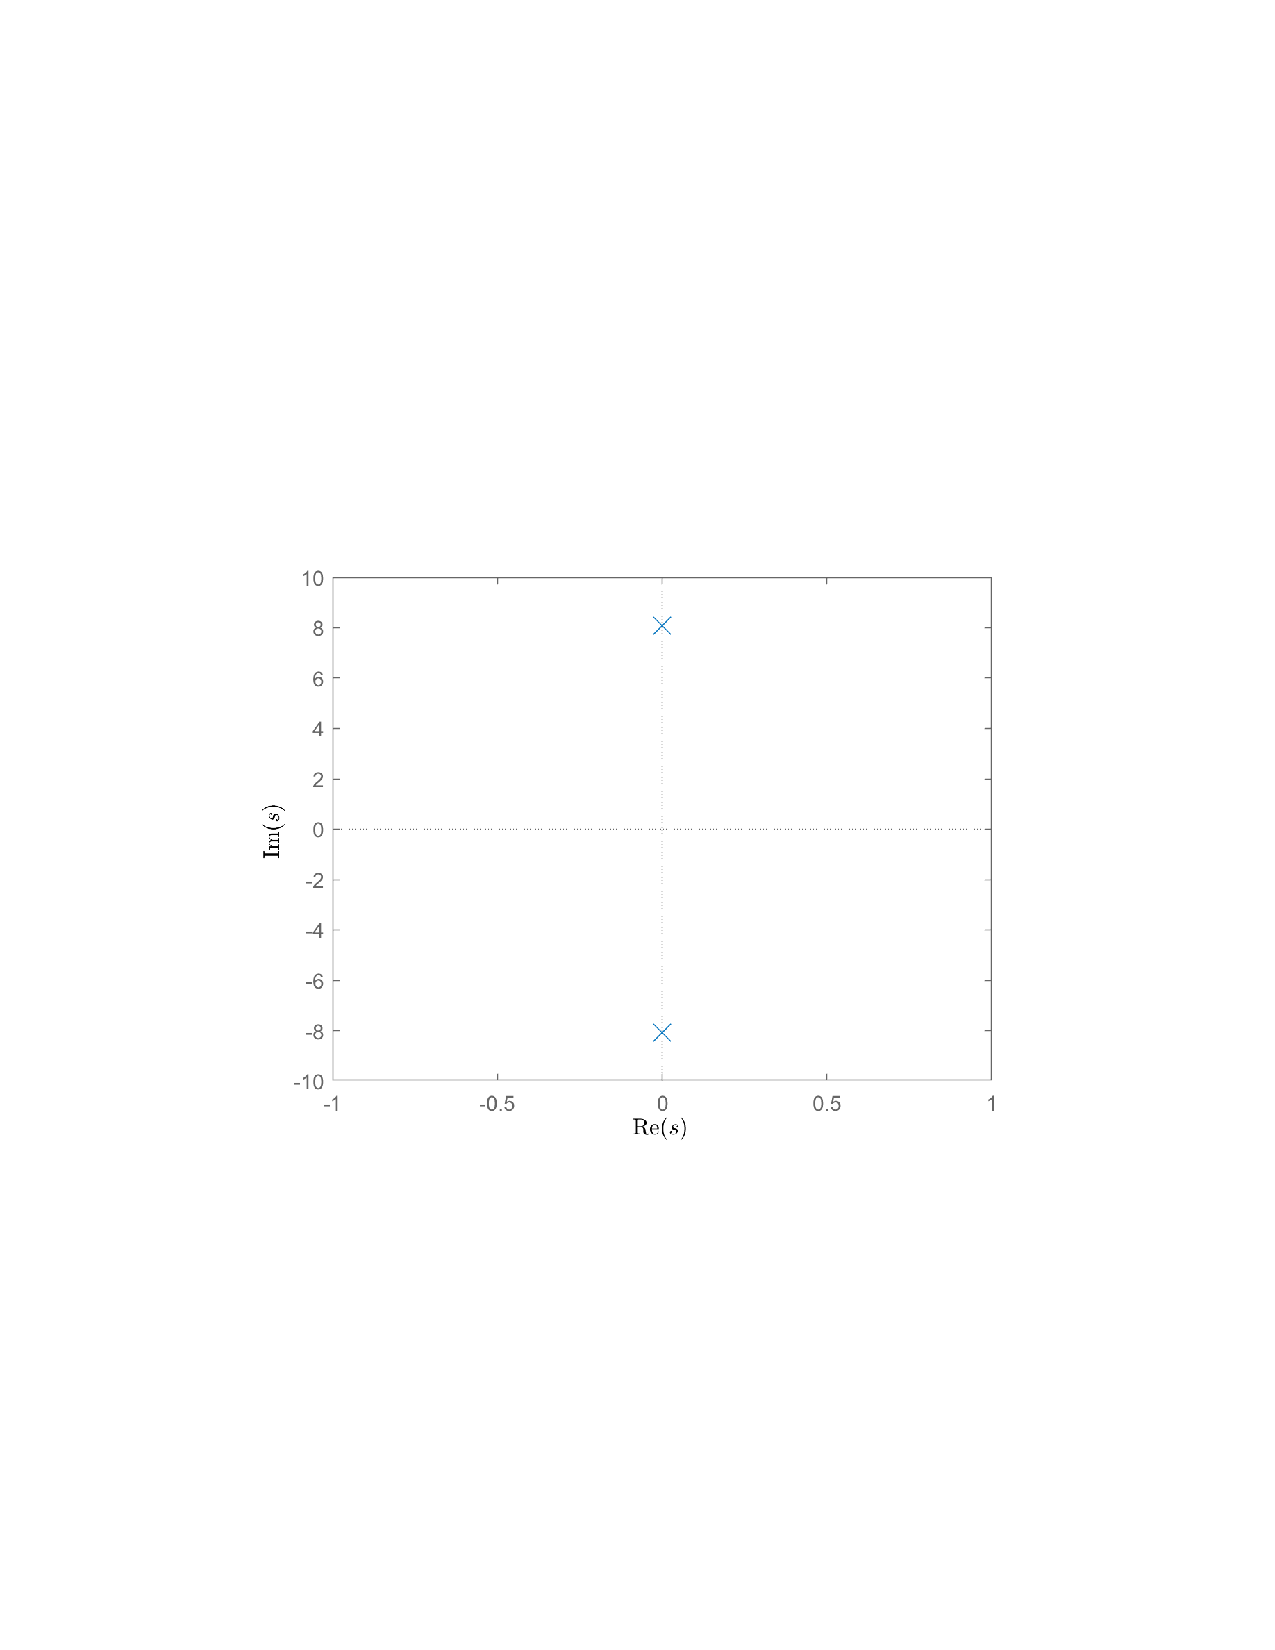
\includegraphics[clip, trim=4.3cm 8.3cm 4.5cm 9.3cm,width=0.45\linewidth]{lab1/figs/section6_pole_zero_gs.pdf}
        \caption{The pole-zero plot for $G(s)$}
\end{figure}

\subsubsection{Input-Output stability}
The system is not BIBO stable as for an input force $u$ that is a sinusoidal with frequency $\approx$ 8.0870 rad/s (the resonance frequency), the transfer function will explode, causing to an unbounded output. This also implies that the system is not I20 stable.

\subsection{Relationship between eigenvalues and frequency of oscillation}
Basically, whenever there is a complex conjugate pair in the eigenvalues of A, the imaginary component results in sinusoidal responses. The imaginary component is what determines the frequency of oscillation, regardless of the value of the real component. This can be verified by graphical inspection, by looking at figures 6 and 8. In 10 seconds, there are 12.5 revolutions, implying that $f = \frac{12.5 \text{ revolutions}}{10 \text{ seconds}}$ but $\omega_n = 2\pi f \approx 7.85$ rad/s $\approx 8.087$ rad/s, which is the imaginary part of the eigenvalue of A.

\section{Controller Design for Pendulum Stabilization}
To now control the pendulum such that for a given initial condition it can converge back to its linearization equilibrium state, which in our case is $\vec{x}_1^*$, we can design a controller, $C(s)$, with (unity-feedback) closed-loop to achieve the objective. For the purpose of the simulation, we can treat the feedback measurement $y_m = y$, the true plant state output.

\begin{figure}[!h]
    \centering
    \mixedcls
    \caption{Closed-loop control system}
\end{figure}

\subsection{Controller Design}
For this system, we were advised to use a lead controller which is of the form, 
\[ C(s) = k\cdot\left(\frac{Ts + 1}{\alpha Ts + 1}\right), \quad \alpha \in (0,1) \text{ and } T,k > 0\]
where $k$ is the dc gain and $1/T$, $1/\alpha T$ are the break frequencies. This is the realizable continuous-time form of a proportional-derivative (PD) controller, particularly between the left and right break frequencies, because of its proper rational transfer function. A PD controller is fit for such a problem since we can make it act as an active damper to make the system take its stable equilibrium of hanging down and being stationary (or moving with a constant velocity).

Now, to extend the approximation of a PD controller over a wide range of frequencies, we need the pole frequency, $1/\alpha T$, much to the right from the zero frequency, $1/T$. This will require that $\alpha \ll 1$. We can then increase the loop gain, $k$, to get better tracking performance by strengthening the proportional term. Since we most need the PD behavior near the natural frequency of the plant, $\omega_n = 8.087$ rad/s, we have set $1/T = 10$ and accordingly chose $\alpha=10^{-5}$ for effective performance over a wide band of frequencies. We considered $k = -30$, as suggested in the lab document, which was sufficient for all test cases. The resulting controller is,

\begin{equation*}
    C(s) = -30\cdot\frac{0.1s+1}{10^{-5}s+1}.
\end{equation*}

Now, considering the stability of the controller, it is important that it abides by the following criteria:

\begin{enumerate}
    \item $1 + L(s)$ has all its zeros in $\mathbb{C}^-$, where $L(s) = C(s)G(s)$. These correspond to the poles in the closed-loop system.
    \item There are no unstable zero-pole cancellations in $L(s)$.
\end{enumerate}

Based on the structure of $C(s)$, we can conclude that criterion 2 is met. We can then write out $L(s)$ to verify criterion 1.

\begin{equation*}
L(s) = \frac{100s + 1000}{10^-5s^3+s^2+0.000654s+65.4}
\end{equation*}

\begin{equation*}
    1+L(s) = \frac{(s + 9.99 \times 10^4)(s+87.97)(s+12.12)}{(s+10^5)(s^2+65.4)}
\end{equation*}

As can be seen above, the zeros of $1+L(s)$ are: $-9.99\cdot 10^4, \quad -0.0088\cdot 10^4, \text{ and } -0.0012\cdot 10^4$ which are all in $\mathbb{C}^-$. The zero-pole plots of $C(s)$ and $1 + L(s)$ can be found below.

\begin{figure}[ht]
    \centering
    \begin{minipage}[b]{0.45\textwidth}
        \centering
        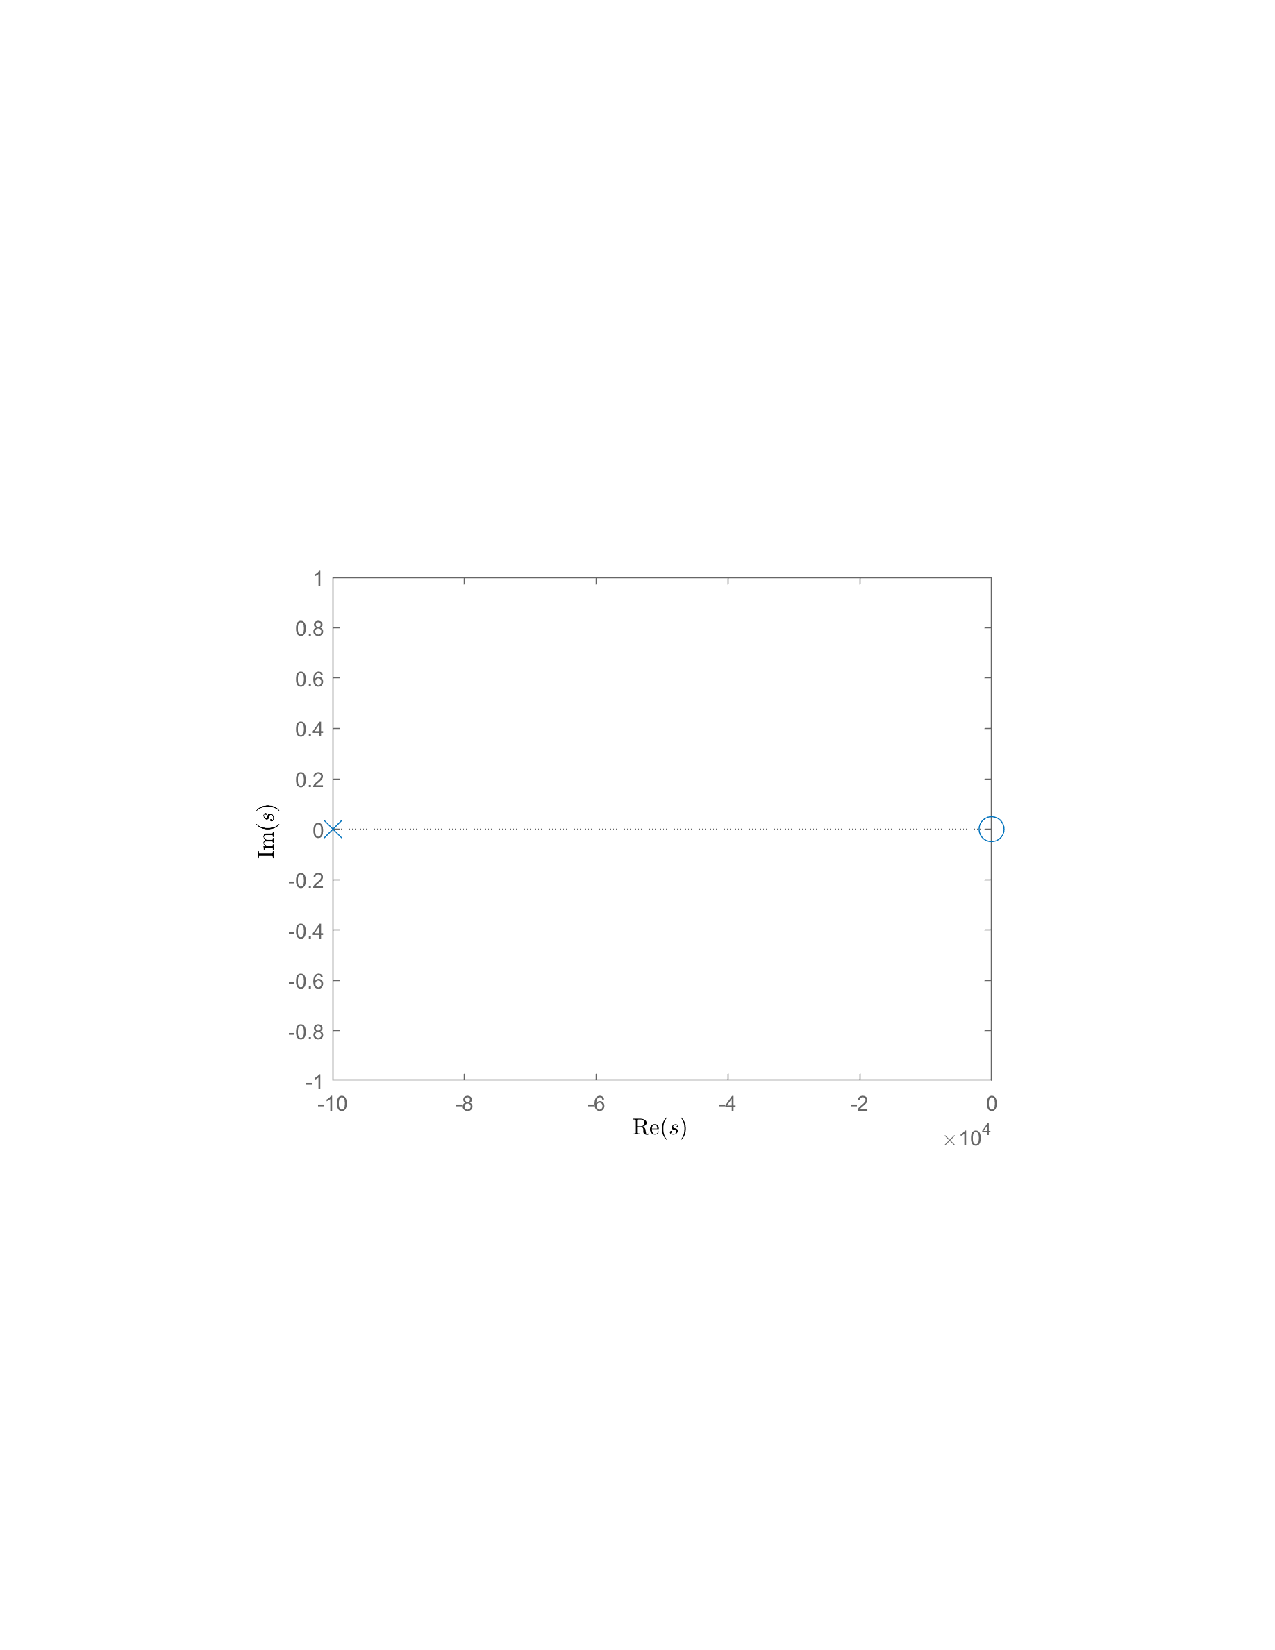
\includegraphics[clip, trim=4.3cm 8.3cm 4.5cm 9.3cm,width=1\linewidth]{lab1/figs/section7_pole_zero_cs.pdf}
        \captionof{figure}{Pole-zero plot for $C(s)$}    
    \end{minipage}
    \begin{minipage}[b]{0.45\textwidth}
        \centering
        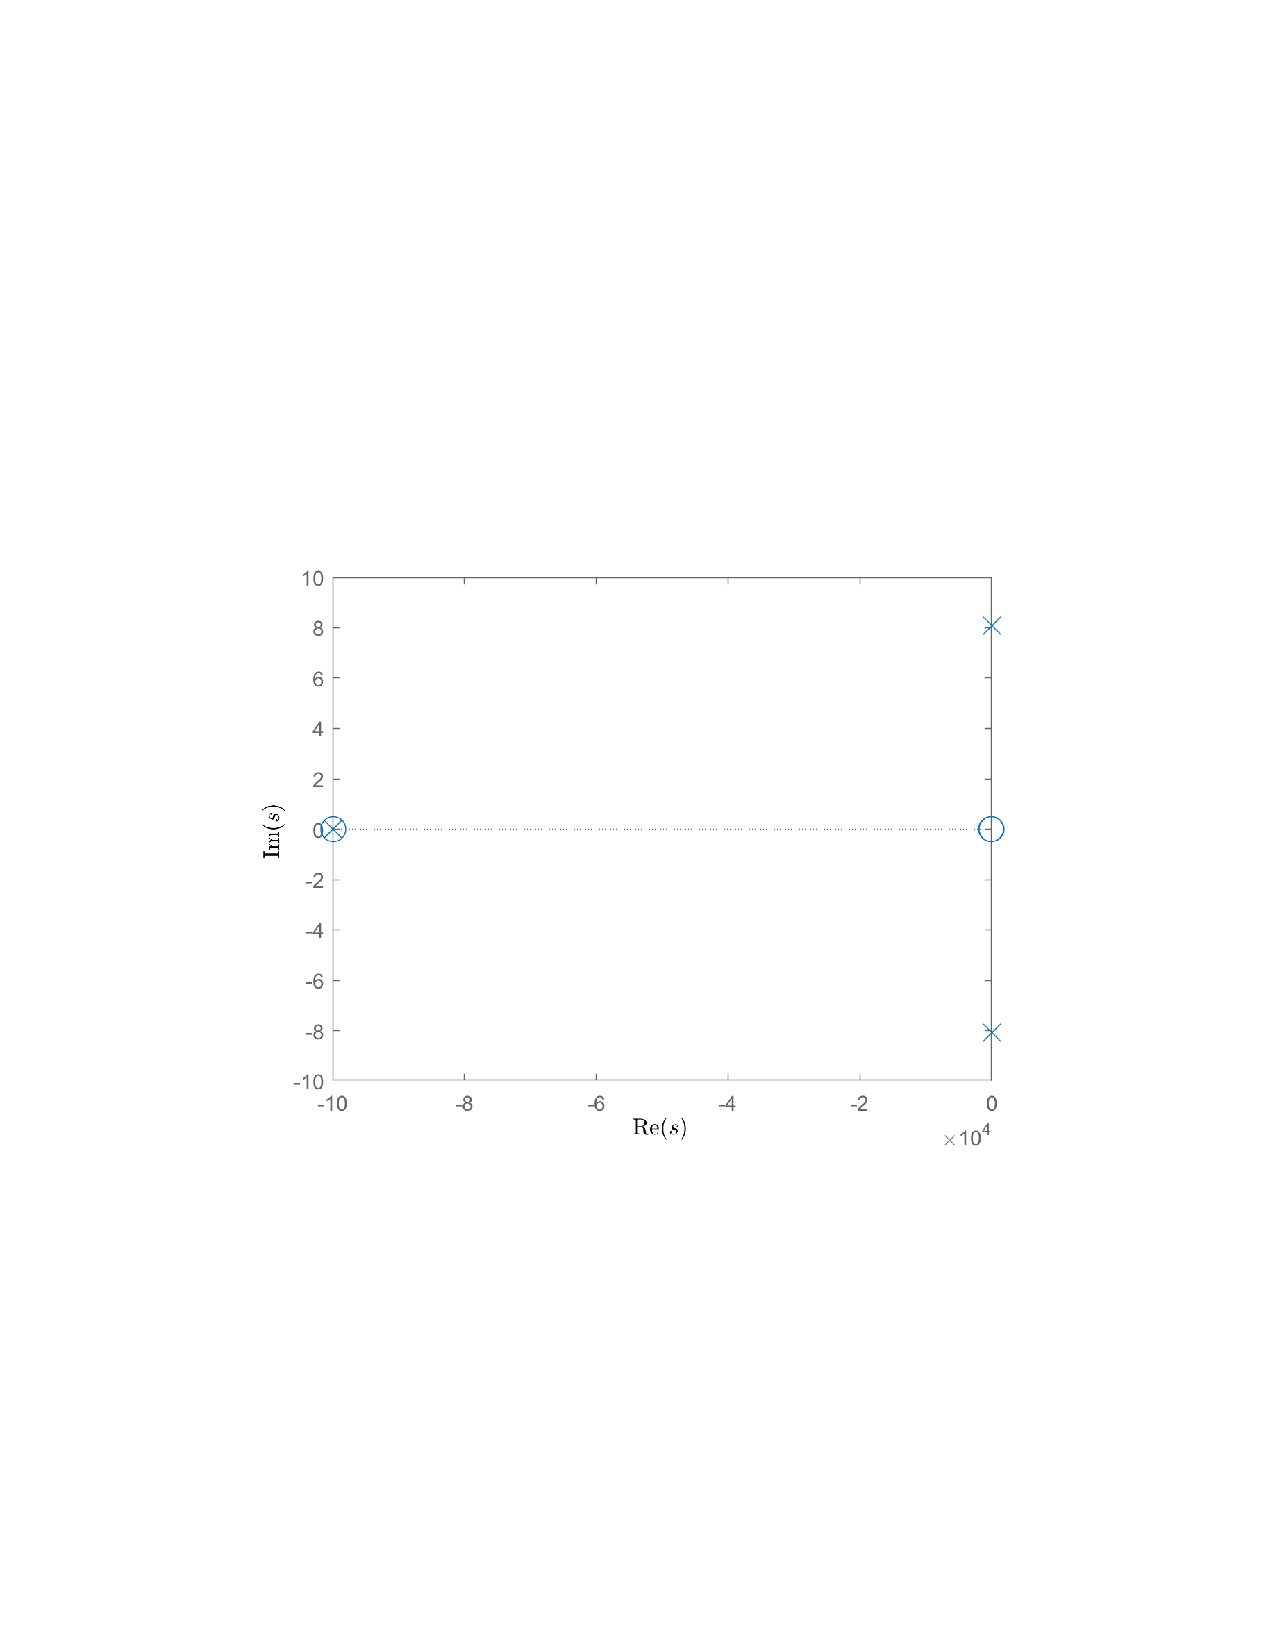
\includegraphics[clip, trim=4.3cm 8.3cm 4.5cm 9.3cm,width=1\linewidth]{lab1/figs/section7_pole_zero_cls.pdf}
        \captionof{figure}{Pole-zero plot for $1+L(s)$}
    \end{minipage}
\end{figure}

\subsection{Pendulum Stabilization}

\subsubsection{Controlled System Response for different initial conditions}
We will now analyse the output of the system (with the controller) for the two initial conditions considered throughout the report. 

\begin{figure}[ht]
    \centering
    \begin{minipage}[b]{0.45\textwidth}
        \centering
        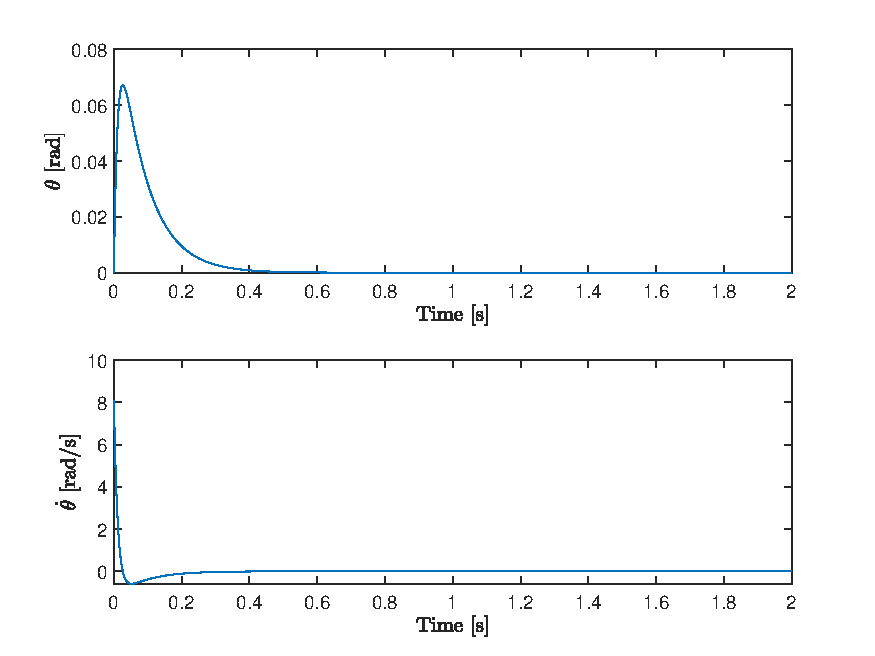
\includegraphics[clip,width=1\linewidth]{lab1/figs/section7_controlled_state_evolution_x_0_1.pdf}
        \captionof{figure}{Controlled State Evolution for $\vec{x}_{0,1}$}    
    \end{minipage}
    \begin{minipage}[b]{0.45\textwidth}
        \centering
        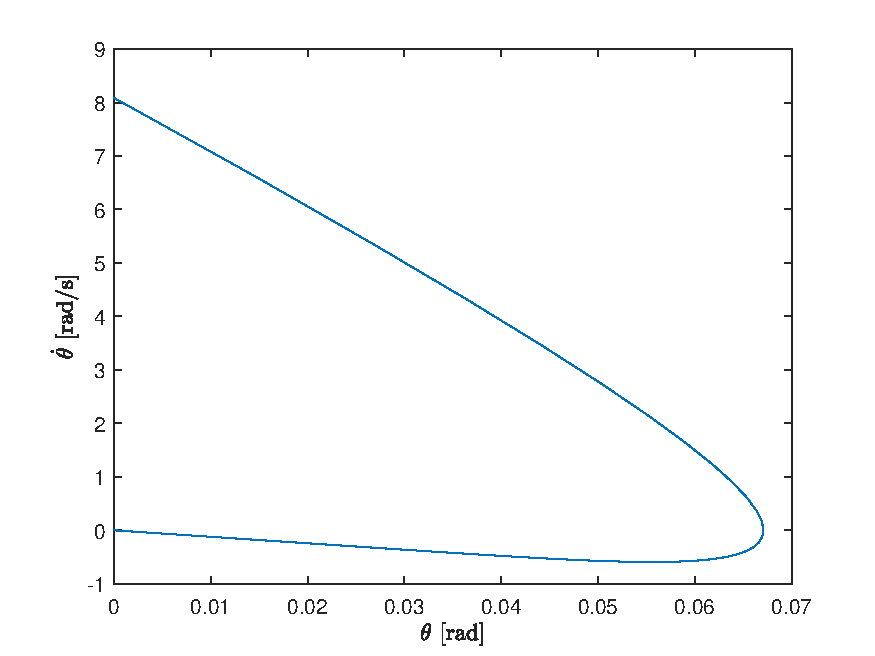
\includegraphics[clip,width=1\linewidth]{lab1/figs/section7_controlled_state_orbit_x_0_1.pdf}
        \captionof{figure}{Controlled State Orbit for $\vec{x}_{0,1}$}
    \end{minipage}
\end{figure}

\begin{figure}[ht]
    \centering
    \begin{minipage}[b]{0.45\textwidth}
        \centering
        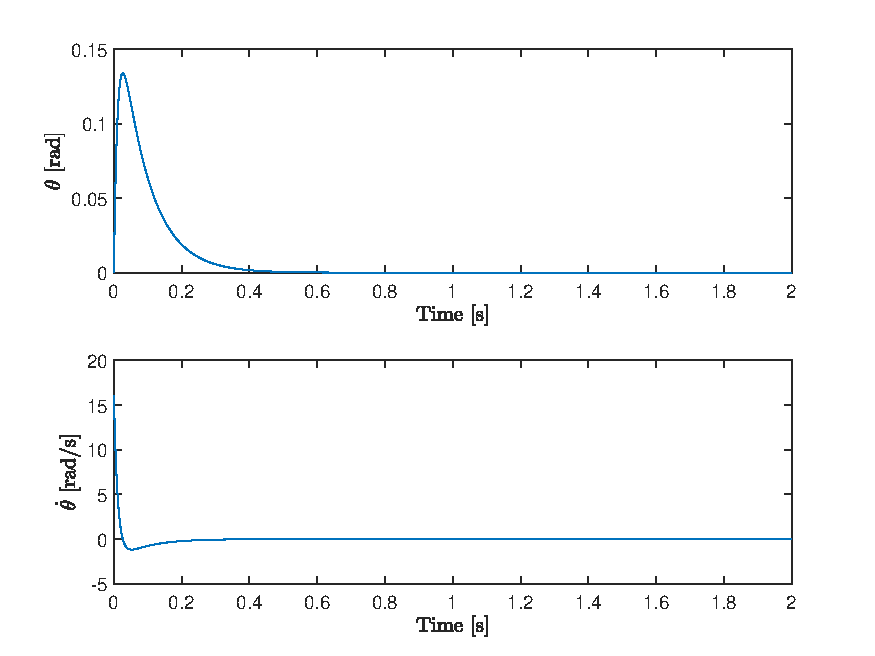
\includegraphics[clip,width=1\linewidth]{lab1/figs/section7_controlled_state_evolution_x_0_2.pdf}
        \captionof{figure}{Controlled State Evolution for $\vec{x}_{0,2}$}    
    \end{minipage}
    \begin{minipage}[b]{0.45\textwidth}
        \centering
        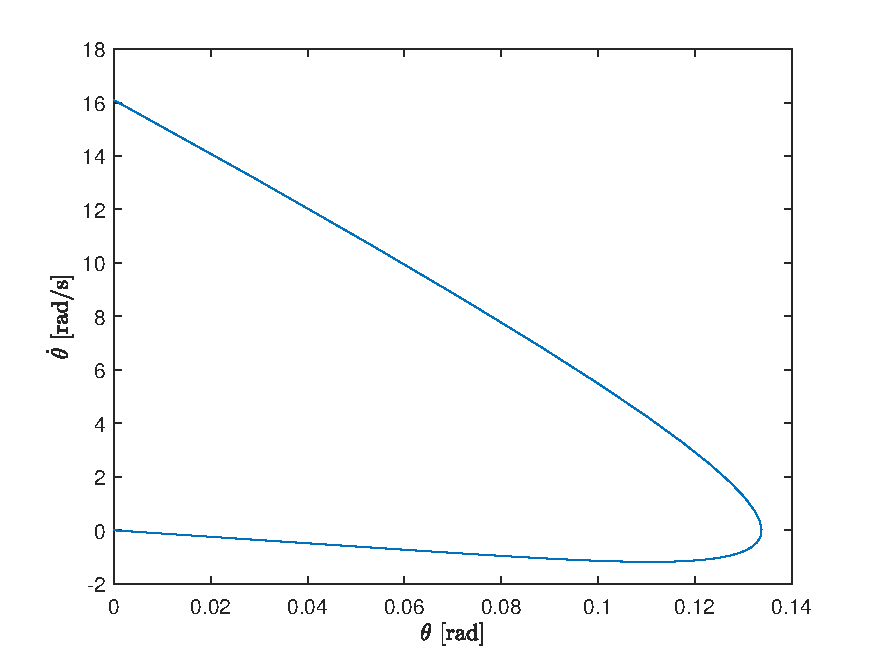
\includegraphics[clip,width=1\linewidth]{lab1/figs/section7_controlled_state_orbit_x_0_2.pdf}
        \captionof{figure}{Controlled State Orbit for $\vec{x}_{0,2}$}
    \end{minipage}
\end{figure}

The system responds to both the initial conditions in a similar manner; i.e., the shape of the state evolution as well as the state orbit is the same for both initial conditions, the only difference being in the range of $\theta$ and $\dot{\theta}$. The controller does a good job of ensuring that the pendulum reaches the equilibrium point without any oscillatory output. Note that both conditions take the same amount of time to reach equilibrium, but the angle swept (and its angular velocity) is greater for initial condition 2 because of the higher energy injected in the system. 

\subsubsection{Control system response for different initial angles $\theta_0$}
Three different initial pendulum angles were picked in the following order $\pi/4, \pi/2, \pi$ to test the controlled system's output. Note, the angular velocity ($\dot{\theta}$) is set to 0 for the following system responses.

\begin{figure}[ht]
    \centering
    \begin{minipage}[b]{0.45\textwidth}
        \centering
        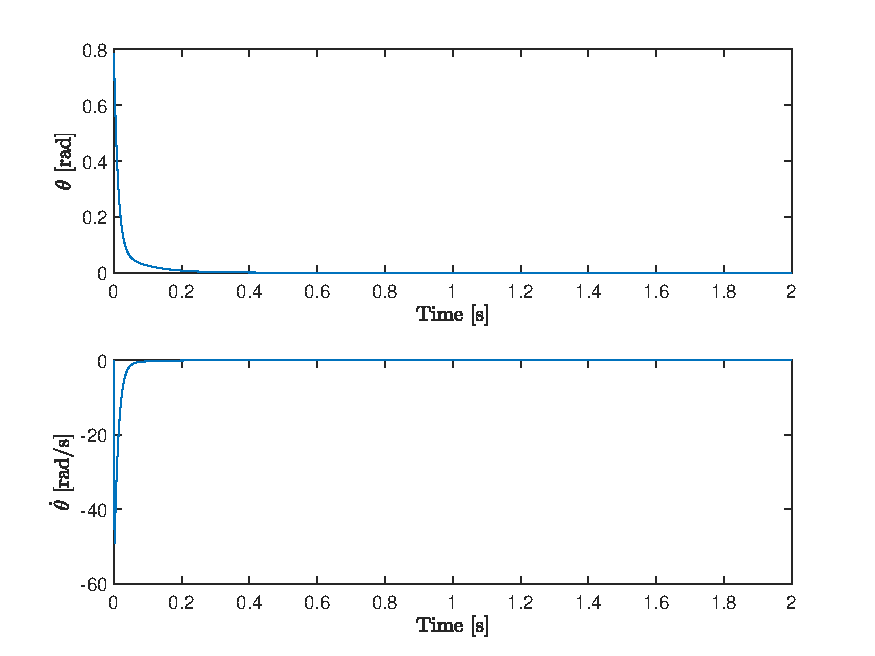
\includegraphics[clip,width=1\linewidth]{lab1/figs/section7_controlled_state_evolution_x_0_3.pdf}
        \captionof{figure}{Controlled State Evolution for $\theta_0 = \frac{\pi}{4}$}    
    \end{minipage}
    \begin{minipage}[b]{0.45\textwidth}
        \centering
        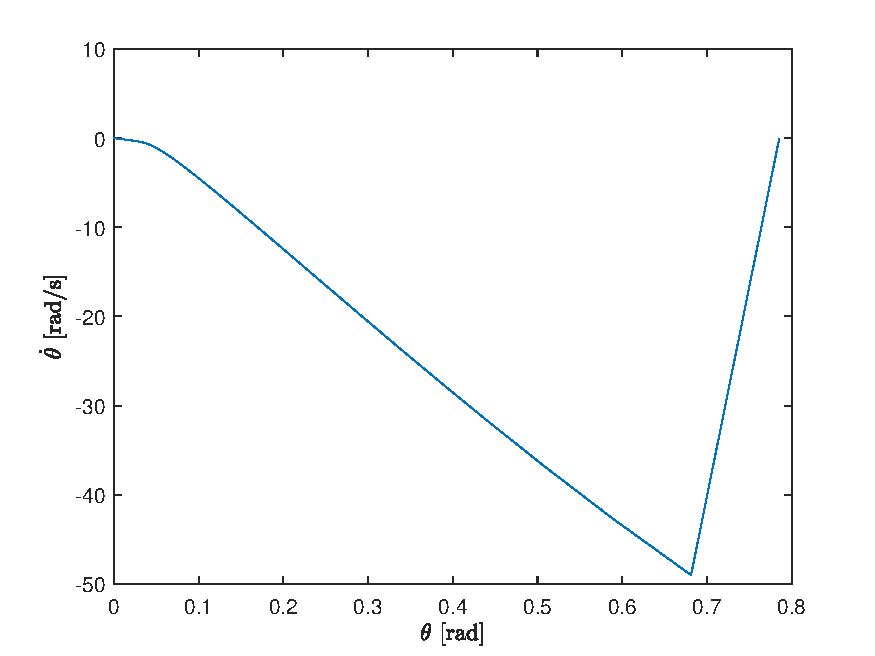
\includegraphics[clip,width=1\linewidth]{lab1/figs/section7_controlled_state_orbit_x_0_3.pdf}
        \captionof{figure}{Controlled State Orbit for $\theta_0 = \frac{\pi}{4}$}
    \end{minipage}
\end{figure}


\begin{figure}[ht]
    \centering
    \begin{minipage}[b]{0.45\textwidth}
        \centering
        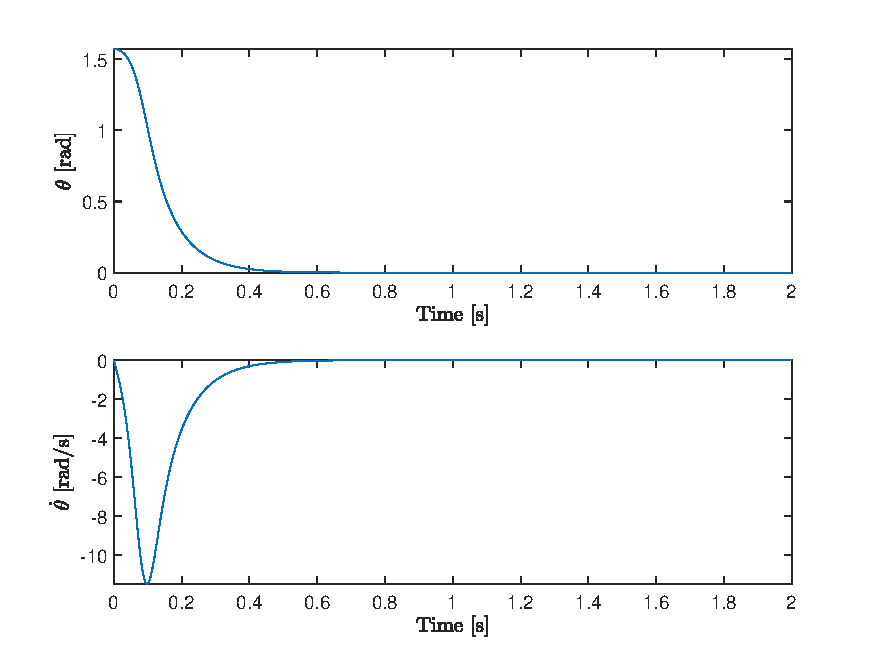
\includegraphics[clip,width=1\linewidth]{lab1/figs/section7_controlled_state_evolution_x_0_4.pdf}
        \captionof{figure}{Controlled State Evolution for $\theta_0 = \frac{\pi}{2}$}
    \end{minipage}
    \begin{minipage}[b]{0.45\textwidth}
        \centering
        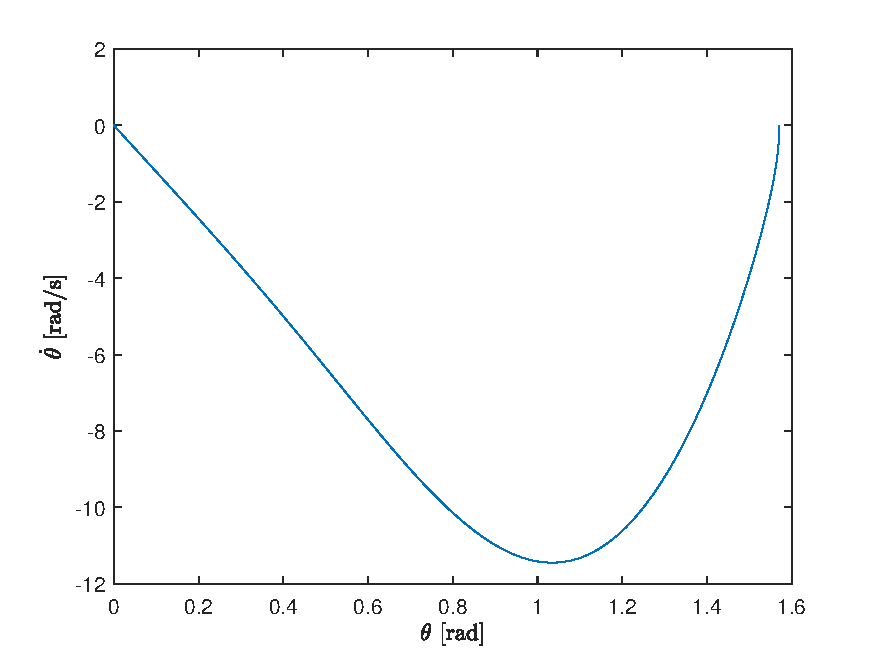
\includegraphics[clip,width=1\linewidth]{lab1/figs/section7_controlled_state_orbit_x_0_4.pdf}
        \captionof{figure}{Controlled State Orbit for $\theta_0 = \frac{\pi}{2}$}
    \end{minipage}
\end{figure}

\begin{figure}[ht]
    \centering
    \begin{minipage}[b]{0.45\textwidth}
        \centering
        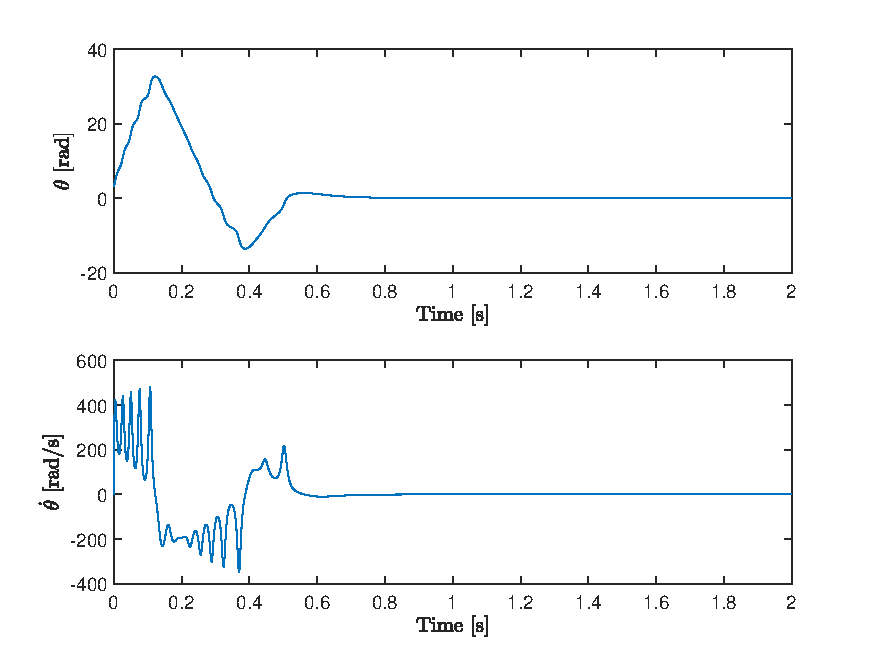
\includegraphics[clip,width=1\linewidth]{lab1/figs/section7_controlled_state_evolution_x_0_5.pdf}
        \captionof{figure}{Controlled State Evolution for $\theta_0 = \pi$}    
    \end{minipage}
    \begin{minipage}[b]{0.45\textwidth}
        \centering
        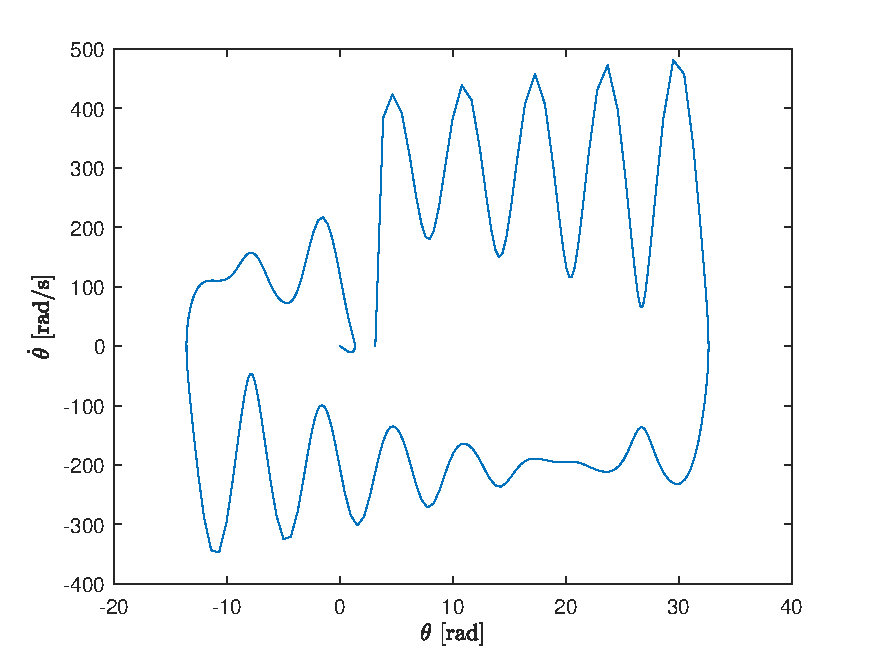
\includegraphics[clip,width=1\linewidth]{lab1/figs/section7_controlled_state_orbit_x_0_5.pdf}
        \captionof{figure}{Controlled State Orbit for $\theta_0 = \pi$}
    \end{minipage}
\end{figure}

Here, despite increasing $\theta_0$, the controller is able to realize the equilibrium. However, the performance of the controller falls as $\theta$ is increased. At smaller angles, the controller is able to reach steady state quickly and without any oscillations. At $\pi$, the performance of the controller is not ideal, as the range for the angles swept are from -10 rad to 30 rad, whereas the controller is only supposed to induce a difference of $\pi$ rad (from $\pi$ to 0 rad). Regardless, the controller design is promising, as it works on the entire spectrum of $\theta$ values. 

\end{document}